\chapter{Stabilitásvizsgálat időkéséssel}\label{chap:time_delay_stability}


% \section{Vizsgálati módszerek összehasonlítása}
% A rúd differenciálegyenlete
% \begin{align}
%     \ddot\phi\left(t\right) - \frac{6g}{l}\phi\left(t\right) + 
%     \frac{6D}{ml}\dot\phi\left(t-\tau\right) + \frac{6P}{ml}\phi\left(t-\tau\right) = 0
% \end{align}
% A differenciálegyenlet Laplace transzformáltja
% \begin{align}
%     s^2\phi\left(s\right) - s\phi_0 - \dot\phi_0 - 
%     \frac{6g}{l}\phi\left(s\right) + 
%     \frac{6D}{ml}\left(se^{-s\tau}\phi\left(s\right)-\phi_{-\tau}\right) + 
%     \frac{6P}{ml}e^{-s\tau}\phi\left(s\right) = 0 
% \end{align}
% Kifejezve $\phi\left(s\right)$-t
% \begin{align}
%     \phi\left(s\right) = \frac{s\phi_0+\dot\phi_0+\frac{6D}{ml}\phi_{-\tau}}{s^2+\frac{6D}{ml}se^{-s\tau}+\frac{6P}{ml}e^{-s\tau}-\frac{6g}{l}}
% \end{align}
% A végérték frekvenciatartománybeli reprezentációban
% \begin{align}
%     \lim_{t \to \infty}\phi\left(t\right) = 
%     \lim_{s \to 0} \phi\left(s\right) = 
%     \frac{\dot\phi_0+\frac{6D}{ml}\phi_{-\tau}}{\frac{6P}{ml}-\frac{6g}{l}}
% \end{align}
% Az időkésést Taylor-sorral közelítve
% \begin{align}
%     \phi\left(t-\tau\right) = \phi\left(t-\right) - 
%     \frac{1}{1!}\dot\phi\left(t\right)\tau + 
%     \frac{1}{2!}\ddot\phi\left(t\right)\tau^2 - 
%     \frac{1}{3!}\dddot\phi\left(t\right)\tau^3 + \ldots
% \end{align}
% különböző rendű közelítéssekkel

\section{Stabilitás folytonos időben}
\begin{figure}[ht]
    \begin{center}
    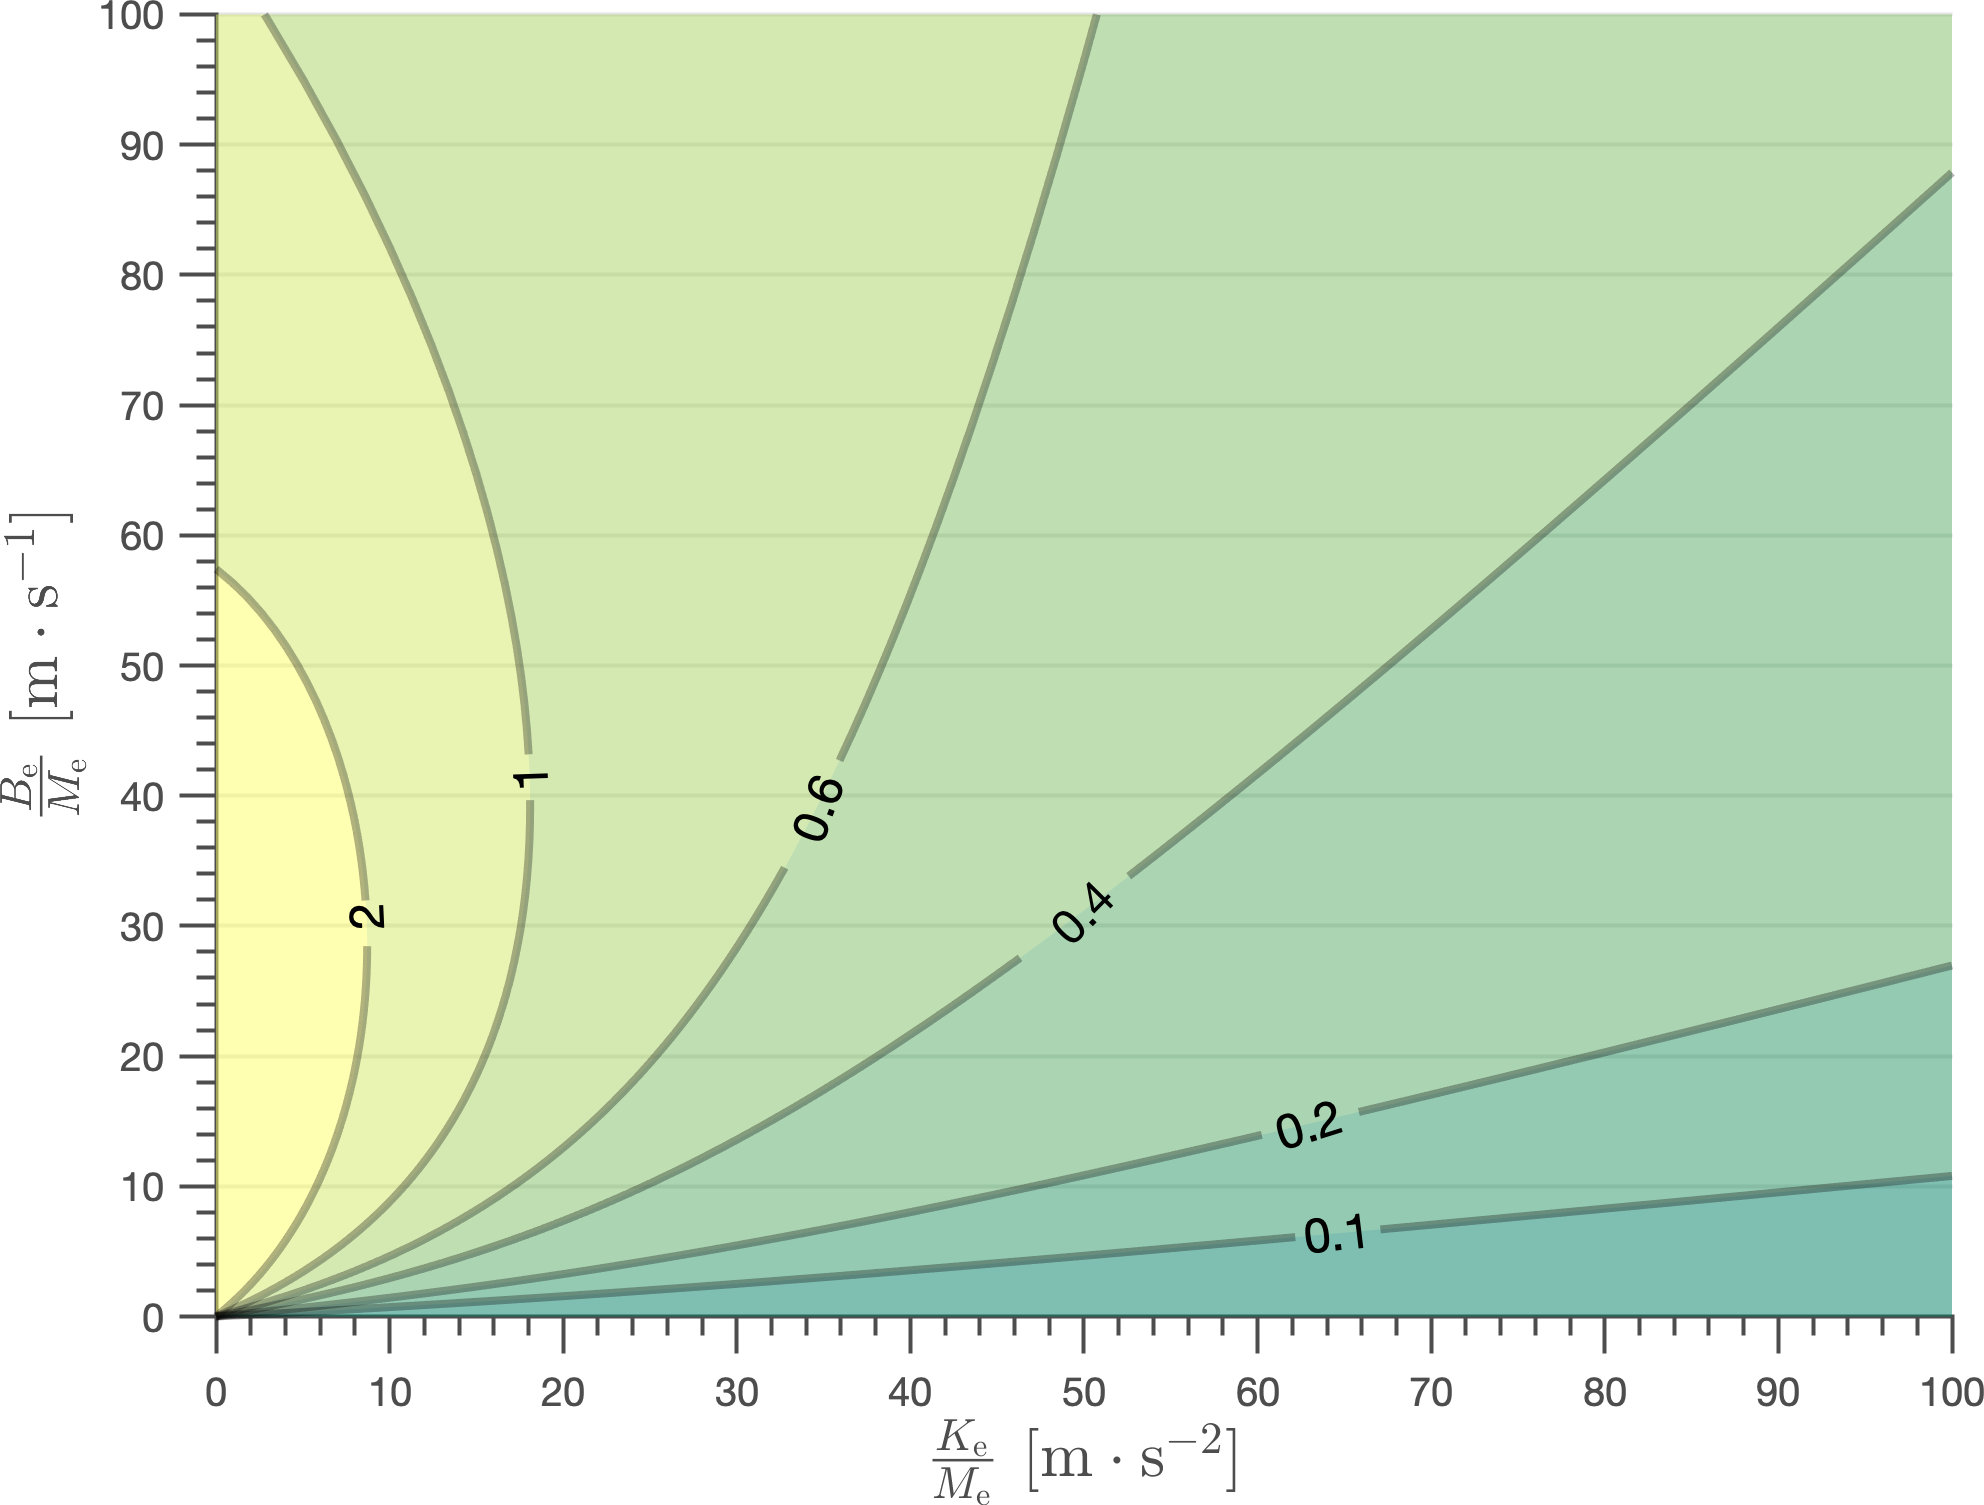
\includegraphics[width=\textwidth]{images/time_delay_stab_map.png}
    \caption{Az előírható tehetetlenség és a független pólus közötti összefüggés}\label{fig:observer_controller_param_limits}
    \end{center}
\end{figure}

\section{Stabilitás diszkrét időben}